\begin{frame}{DSPIGCN couples motion streams through a polynomial}
\framesubtitle{YAN Zhengyang | Independent implementation}
\begin{itemize}
\item Displacement and velocity: separate temporal attention, GCN and TCN.
\item Degree-four $P(t)$ links predicted positions to velocities through $P'(t)$.
\item Gaussian likelihood + squared reconstruction + physical residual.
\item History-only inputs; independently tested units, gradients and causality.
\end{itemize}
\small Guo et al., KDD 2026. Registered departures: target-centered positions,
3 m history context and residual initialization. No copied model core.
\end{frame}

\begin{frame}{Twenty paths cover a range of outcomes}
\centering
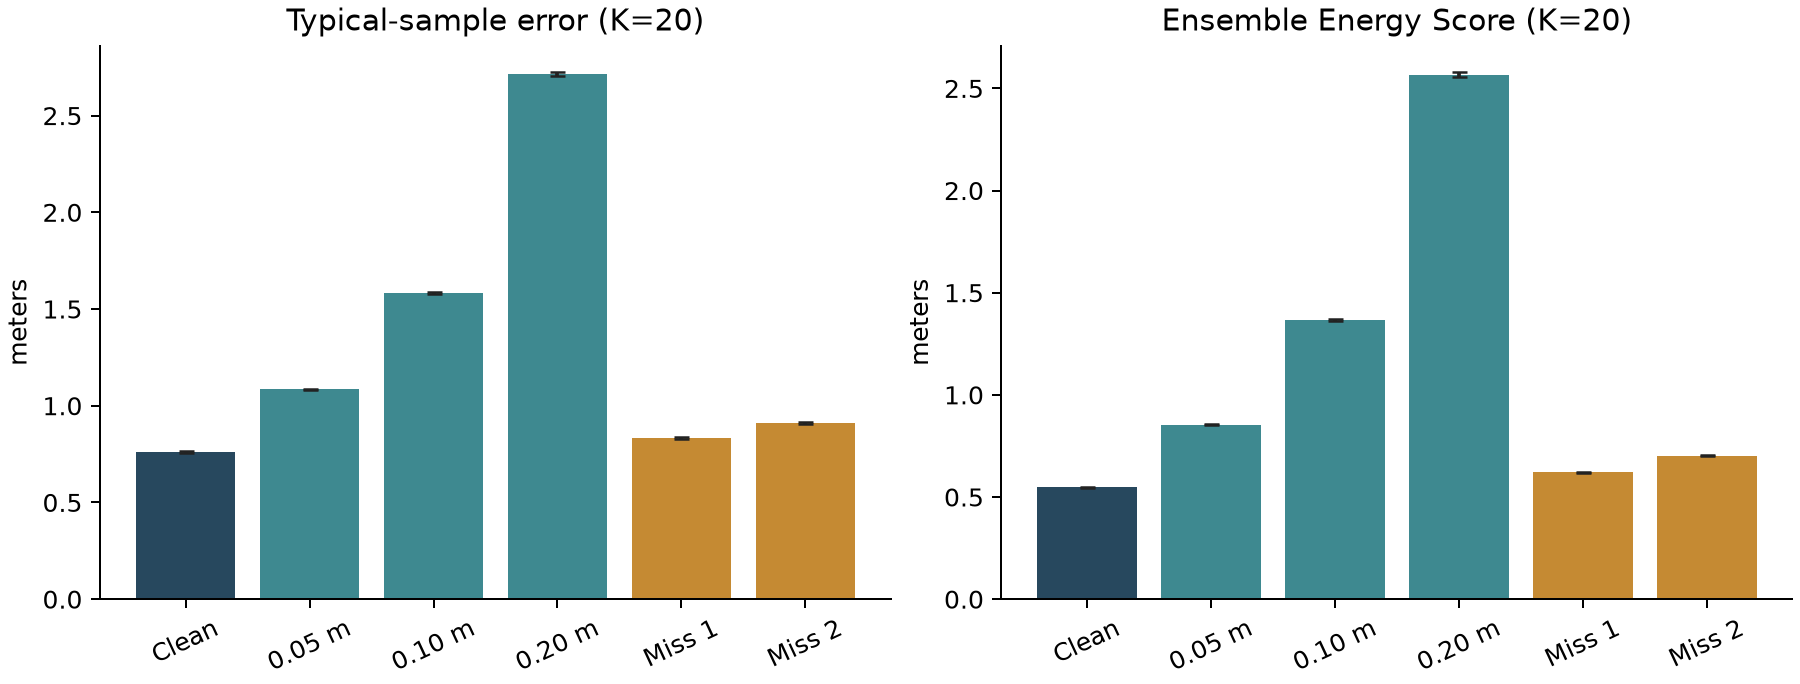
\includegraphics[width=.93\linewidth,height=.62\textheight,keepaspectratio]{contributions/dspigcn/assets/robustness.png}\par
\small On clean histories the best draw has ADE
\ModelMetric{dspigcn}{clean_0}{min_ade_mean}\,m. Averaging all draws gives
\ModelMetric{dspigcn}{clean_0}{mean_ade_mean}\,m. The five holdouts have equal weight.
\end{frame}

\begin{frame}{One ETH pedestrian under three observation conditions}
\centering
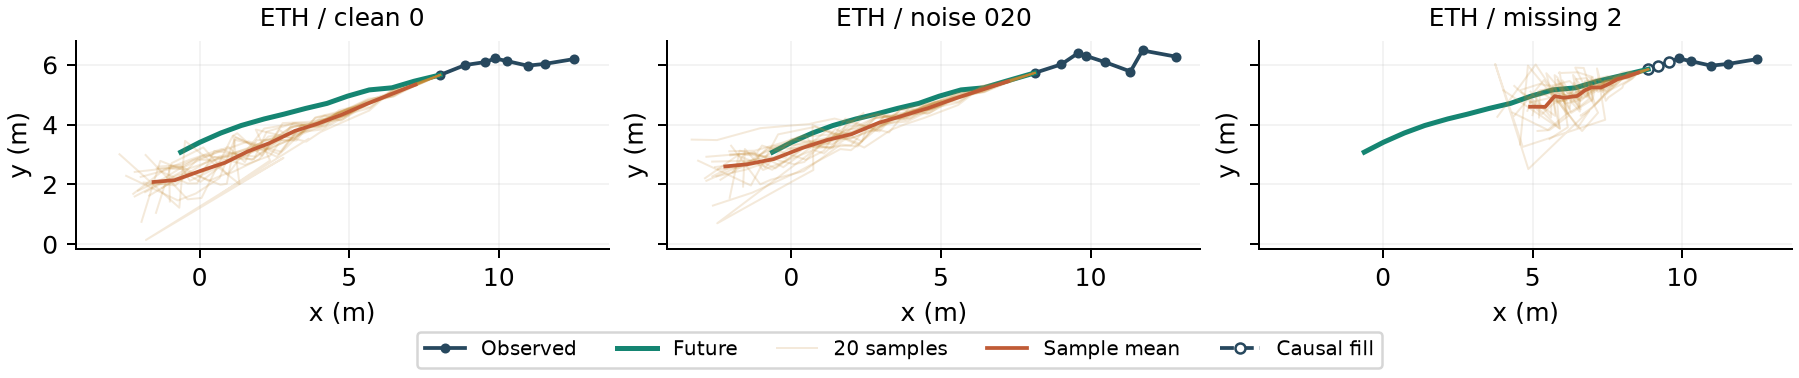
\includegraphics[width=.96\linewidth,height=.60\textheight,keepaspectratio]{contributions/dspigcn/assets/fixed_eth.png}\par
\small Each panel shows the same target, weights and twenty random draws.
Only the target's eight observed positions are perturbed or filled.
\end{frame}
